\documentclass[a4paper, twocolumn,
final
%draft
]{article}

\usepackage[top=1.5cm,bottom=2cm,left=1.5cm,right=1.5cm]{geometry}

\usepackage{url}
\usepackage{microtype}
\usepackage{color}
\pagestyle{empty}

% Use utf-8 encoding for foreign characters
\usepackage[utf8]{inputenc}
\usepackage[T1]{fontenc}

% Setup for fullpage use
%\usepackage{fullpage}
\usepackage[ngerman,british, english]{babel}
% Uncomment some of the following if you use the features
%
% Running Headers and footers
\usepackage{fancyhdr}

% Multipart figures
\usepackage{subfigure}

% More symbols
%\usepackage{amsmath}
%\usepackage{amssymb}
%\usepackage{latexsym}

% Surround parts of graphics with box
\usepackage{boxedminipage}

% Package for including code in the document
\usepackage{listings}

% If you want to generate a toc for each chapter (use with book)
\usepackage{minitoc}

% This is now the recommended way for checking for PDFLaTeX:
\usepackage{ifpdf}

\ifpdf
\usepackage[pdftex]{graphicx}
\else
\usepackage{graphicx}
\fi

\title{TODO: TITLE}
\author{Andreas Ergenzinger and Josua Krause}

\date{\today}
\selectlanguage{english}

\newcommand{\todo}[1]{\colorbox{red}{\textbf{TODO} #1}}
\newcommand{\figref}[1]{Figure~\ref{fig:#1}}
\newcommand*{\vcenteredhbox}[1]{\begingroup
\setbox0=\hbox{#1}\parbox{\wd0}{\box0}\endgroup}

\begin{document}
\maketitle
\thispagestyle{empty}

\section*{Introduction}
We present \emph{BeGIS}, a geographic information system
showcasing various presentation techniques exemplified with
data centered around the city Berlin.
The application uses a zoomable user-interface provided
by the cartography organization open-street maps and overlays
additional information on top of the map.
The real-world dataset is
attributed with position data and shows functionalities of
our tool by solving given tasks.

Following we present the tasks which are divided into
hard and soft tasks. The hard tasks show basic capabilities
of our tool while the soft tasks allow for more freedom
and present extended functionality.

\section*{Hard Tasks}
Our tool allows to show certain objects attributed with
geographic positions, like buildings, parks, waters, districts, and
photos taken in Berlin.
The user can click on each pair of those objects to get information about
relationships between them.
The tool takes the type of object into account and displays, according
to feasibility, the minimal distance between the objects, whether they lie
inside of each other, and how the objects intersect following the 9-cut model.

The photos from the website Flickr are all tagged as Brandenburg gate.
Therefore, we show them as points with a size proportional to
the distance to the landmark.
Hovering over a photo displays the picture next to the mouse
as seen in \figref{brandenburg}.

\begin{figure}[b]
\centering
\includegraphics[width=0.9\linewidth]{imgs/brand}
\caption{Photos tagged as Brandenburg gate. The size of the dots
is proportional to the distance to the actual landmark.
A hovered photo shows the actual picture.}
\label{fig:brandenburg}
\end{figure}

Choropleth maps show the ratio of the areas of commercial buildings to their surrounding
district (\figref{commercial}) and the relative amount of
Flickr photos in a district (\figref{flickr}).
\figref{parks} shows parks and whether they are near water.
\begin{figure}
        \centering
		\includegraphics[width=0.6\linewidth]{imgs/commercial}
        \caption{A choropleth map showing the ratio of the area of commercial buildings
        per district to the area of the district.}
		\label{fig:commercial}
\end{figure}
An overlay (\figref{museum}) shows proximity to the nearest museum mapped as color.
We modified the standard scan-line approach of calculating the distance field to
increase accuracy while maintaining computation time. This is done by storing
the nearest museum in every pixel and computing the distance after the standard
algorithm has finished. This gives a smoother result. By searching for the nearest
museum in all border pixels of the result image before the algorithm, museums that
are not within the view-port can be taken into account, which is not possible with
the standard algorithm.

\begin{figure}[b]
        \centering
		\includegraphics[width=0.4\linewidth]{imgs/museum}
        \caption{Showing distances to nearby museums encoded as color. White regions
        are near to a museum and green areas are further away than $500m$ to the
        nearest museum.}
		\label{fig:museum}
\end{figure}
\begin{figure*}[t]
		\centering
		\begin{subfigure}[b]{0.25\textwidth}
                \centering
                \includegraphics[width=\textwidth]{imgs/flickr}
                \caption{A choropleth map showing the relative amount of flickr photos tagged
                as Brandenburg gate in a given district.}
                \label{fig:flickr}
        \end{subfigure}
        \hspace*{0.02\textwidth}
        \begin{subfigure}[b]{0.25\textwidth}
				\centering
				\includegraphics[width=\textwidth]{imgs/rel}
				\caption{A selection of two districts showing the message that
				they meet along with the corresponding 9-cut matrix.}
				\label{fig:rel}
		\end{subfigure}
		\hspace*{0.02\textwidth}
        \begin{subfigure}[b]{0.25\textwidth}
                \centering
                \includegraphics[width=\textwidth]{imgs/parks}
                \caption{Blue points are parks near water. Beige points represent parks further
                away from water than $50m$.}
                \label{fig:parks}
        \end{subfigure}
        \caption{Some solutions for hard tasks.}
\end{figure*}

\section*{Pub Crawl}
To investigate correlations in the OSM dataset, we provide a combined visualization
called \emph{Pub Crawl}
which shows the average minimum inter-pub distance and the average
minimum pub to ATM distance within each administrative area.
The two dimensions are mapped to hue
and saturation respectively, allowing to visualize them as
choropleth map (\figref{crawl}).
The two measures do not seem to be strongly correlated, but the visualization might
be helpful for anyone planning to go bar-hopping in Berlin.
\begin{figure}[b]
\centering
\includegraphics[width=0.6\linewidth]{imgs/crawl}
\caption{\emph{Pub Crawl} showing inter-pub distances 
and the average minimum pub to ATM distance.}
\label{fig:crawl}
\end{figure}
\section*{Open Wi-Fi}
As additional dataset we use data of open Wi-Fi hotspots in
the area of Berlin.
The data is displayed as a heatmap.

The dataset originally consisted only of plain-text street addresses
of public institutions, hotels, bars, restaurants, coffee places, and
other businesses with open Wi-Fi hotspots.
With the Google geocoding API we retrieved street addresses for all buildings
from the given dataset.
Next, we assigned Hotspots to buildings by matching addresses between the two datasets.

The heatmap is computed in a mesh of
arbitrary size. Each cell is computed by adding
the nearest distances of all buildings with a
hotspot together.
Since this is computationally expensive
we start with a loose mesh and refine it up to one pixel per cell while the
user is inactive.

Looking at the heatmap reveals some areas with higher density of open hotspots.
Namely the center of the city (Mitte), around the Sony Center,
in Prenzlauer Berg, and the area around Simon-Dach-Str.
and around Kürfürstendamm.
Those areas are known for being touristic and Mitte with Sony Center are additionally
areas with many businessmen.
As hotspots are likely to be in a restaurant, bar, or caf\'{e}
this seems to be due to the high demand for internet
from tourists (having no alternative) and businessmen (needing to
be online during lunch).
\begin{figure}
\centering
\includegraphics[width=0.45\linewidth]{imgs/heat}
\caption{The heatmap of free hotspots in Berlin.
The white spot to the right is the area around Simon-Dach-Str.}
\label{fig:heat}
\end{figure}
Based on our visualization of the hotspot data, we hypothesized that the hotspot locations
are unevenly distributed, with a greater density near the city center.
To investigate this further, we computed a distribution of the hotspots w.r.t. their
distance from the centroid of Berlin and compared it to the distribution that would
result from a uniform hotspot density all over Berlin. Both distributions are visualized
as step functions in \figref{wifi_distributions}. Although this simple approach does
not permit conclusions regarding the significance of the apparent differences,
it does support our hypothesis.
\begin{figure}[h]
	\centering
	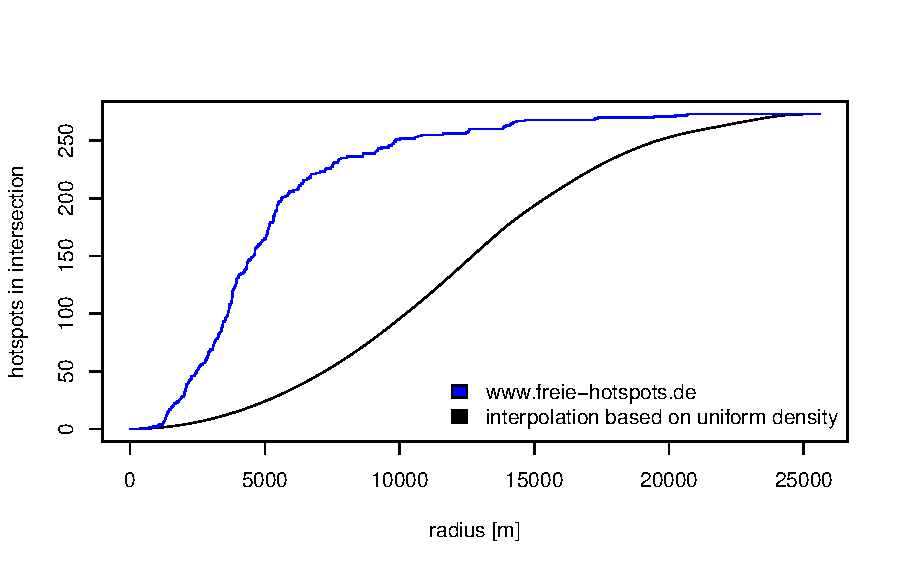
\includegraphics[scale=0.35]{imgs/wifi_distributions.pdf}
	\caption{Number of hotspots within the centroid of Berlin.}
	\label{fig:wifi_distributions}
\end{figure}

\section*{Authors' Contributions}

\begin{description}
\setlength{\itemsep}{0pt}
  \item[Andreas Ergenzinger] Database, distance map, pub crawl, hotspot distribution
  \item[Josua Krause] Graphics efficiency, caching, heatmap, Flickr pictures
\end{description}

\section*{References}

\begin{description}
\setlength{\itemsep}{0pt}
\item[Wi-Fi Positions.]
  \url{http://www.freie-hotspots.de}
\item[Google Geocoding API.]
  \url{https://developers.google.com/maps/documentation/geocoding/}
\end{description}


\bibliography{main}

\end{document}
